\chapter{Reduced descriptions of collections of
  networks \label{ch:graphs}}

% \abstract{In order to illustrate the adaptation of traditional
% continuum numerical techniques to the study of complex network
% systems, we use the equation-free framework to analyze a dynamically
% evolving multigraph.
% %
% This approach is based on coupling short intervals of direct dynamic
% network simulation with appropriately-defined lifting and
% restriction operators, mapping the detailed network description to
% suitable macroscopic (coarse-grained) variables and back.
% %
% This enables the acceleration of direct simulations through Coarse
% Projective Integration (CPI), as well as the identification of
% coarse stationary states via a Newton-GMRES method.
% %
% We also demonstrate the use of data-mining, both linear (principal
% component analysis, PCA) and nonlinear (diffusion maps, DMAPS) to
% determine good macroscopic variables (observables) through which one
% can coarse-grain the model.
% %
% These results suggest methods for decreasing simulation times of
% dynamic real-world systems such as epidemiological network
% models. Additionally, the data-mining techniques could be applied to
% a diverse class of problems to search for a succint, low-dimensional
% description of the system in a small number of variables.}


\section{Introduction\label{sec:intro}}
  

Over the past decades, complex networks have been used as the model of
choice for a truly broad class of physical problems, ranging from
highway traffic \cite{joubert_large-scale_2010} to brain connectivity
\cite{hermundstad_learning_2011}.
%
When modeling such systems, dynamics are typically defined at a very
detailed, ``fine'' scale, specifying individual node and edge
interactions; explicit closed equations governing network macroscopic
(collective) properties are often unavailable
\cite{durrett_graph_2012,joubert_large-scale_2010,roche_agent-based_2011,swaminathan_modeling_1998}.
%
The detailed interactions are often complicated functions dependent on
multiple system parameters, which, when one also accounts for large
network sizes inherent in many interesting problems, can make
systematic numerical exploration computationally prohibitive.
%
The lack of \textit{explicit} macroscopic equations prohibits the use
of traditional numerical techniques such as fixed-point computation
and stability analysis, that could offer valuable insight into the
network's behavior, leaving little alternative but to work with full
direct simulations of the entire network.
%
Faced with these inherent limitations, investigators must either
restrict their attention to a more modest parameter space
\cite{hodgkin_quantitative_1952} or simplify the network model,
potentially removing important features
\cite{brown_variability_1999}. \par

Equation-free modeling offers a promise to circumvent these
challenges, allowing one to investigate the complex network at a
macroscopic level while retaining the effects of full system details
\cite{kevrekidis_equation-free:_2004,gear_equation-free_2003}.
%
Underlying this method is the assumption that, although we cannot
analytically derive equations governing network evolution, such closed
equations do, in principle, exist.
%
Furthermore, these unavailable equations are assumed to involve a
small number of dominant collective (coarse-grained) variables.
%
The important features of the complete network can be in fact, by this
assumption, well represented by these select observable quantities.
%
This may seem too restrictive, yet it is exactly the behavior
witnessed across many network types: despite the initial complexity of
the full system configuration, certain collective network properties
appear to evolve smoothly in time, while the evolution of other,
``secondary'' properties, can be strongly correlated with that of the
few ``primary'' variables
\cite{bold_equation-free_2014,rajendran_coarse_2011,siettos_equation-free_2011}.
%
Once these significant variables are uncovered, we can combine short
intervals of full system simulation with operators that map the full
system description to and from its representative coarse variable
``summary'', thus enabling previously-infeasible system-level analysis
(see Section \ref{sec:ef} for further details). \par

Here, we apply this framework to a dynamically evolving multigraph
model.
%
This offers a test of the methodology in the previously unexplored
context of multigraphs.
%
We demonstrate the acceleration of direct network simulations through
Coarse Projective Integration (CPI), and the location of coarse
stationary states through a matrix-free Newton-GMRES method.
%
In addition, principal component analysis (PCA) and diffusion maps
(DMAPS), two well established dimensionality-reduction techniques, are
shown to enable an algorithm for characterization of the underlying
low-dimensional behavior of the system. \par

The paper is organized as follows: we begin in Section \ref{sec:m}
with a description of the multigraph dynamic model.
%
Sections \ref{sec:ef} and \ref{sec:ng} provide most details of the
equation-free approach, specify how it was applied to our system, and
present subsequent results.
%
Section \ref{sec:dr} summarizes our use of PCA and DMAPS, and assesses
their effectiveness in analyzing hidden, low-dimensional structure in
this network system.

\section{Model description\label{sec:m}}

We study the edge-conservative preferential attachment model, a
detailed mathematical analysis of which can be found in
\cite{rath_time_2012} and \cite{rath_multigraph_2012}.
%
The system evolves in discrete steps $t = 0,1,\ldots t_f$, and we
denote the $n$-vertex graph at each point by $G_n(t)$.
%
The initial state, $G_n(0)$, is an arbitrary distribution of $m$ edges
among the $n$ vertices; the total number of both edges and vertices is
conserved.
%
No restrictions are placed on this initial distribution: multiple
edges and loops are permitted.  The system is then advanced
step-by-step based on the following procedure:

\begin{enumerate}
\item Choose an edge $e_{ij} \in E(G)$ uniformly at random, and flip a
  coin to label one of the ends as $v_{i}$
\item Choose a vertex $v_{k}$ using linear preferential attachment:
  $P(v_{k} = v_{l}) = \frac{d_{l} + \kappa}{\sum\limits_{i=1}^{n}
    d_{i} + n \kappa}$
  \label{step:prob}
\item Replace $e_{ij}$ with $e_{ik}$,
\end{enumerate}

\noindent where $d_i$ is the degree of vertex $v_i$, $E(G)$ is the set
of edges in the graph, and $\kappa \in (0, \infty)$ is a model
parameter affecting the influence degrees have on the probability
distribution in Step \ref{step:prob}.
%
That is, taking $\lim\limits{\kappa \rightarrow 0}$, we recover
``pure'' preferential attachment, and probability scales directly with
degree, while
$\lim\limits_{\kappa \rightarrow \infty} P(v_k = v_l) = \frac{1}{n} \;
\forall \; l$, and individual degrees have no effect. A single step of
this evolution process is illustrated in
Fig. ({\ref{fig:step-illustration}}). Note that this can also be
represented as a graph in which only one edge is permitted between
each pair of nodes, but with edge weights signifying the number, or
strength, of connections between nodes.
\par

Evolving the system in this manner, the degree sequence approaches a
stationary distribution over $O(n^3)$ steps.
%
As explained in \cite{rath_time_2012}, this distribution is dependent
only on the system parameters $\rho = \frac{2*m}{n}$ and $\kappa$.
%
Fig. (\ref{fig:dse}) illustrates the evolution of the degree sequence
of two networks with different initial configurations but the same
values of $\rho$ and $\kappa$ respectively; as expected, we observe
they approach an identical stationary state.

  \begin{figure}
    \centering
    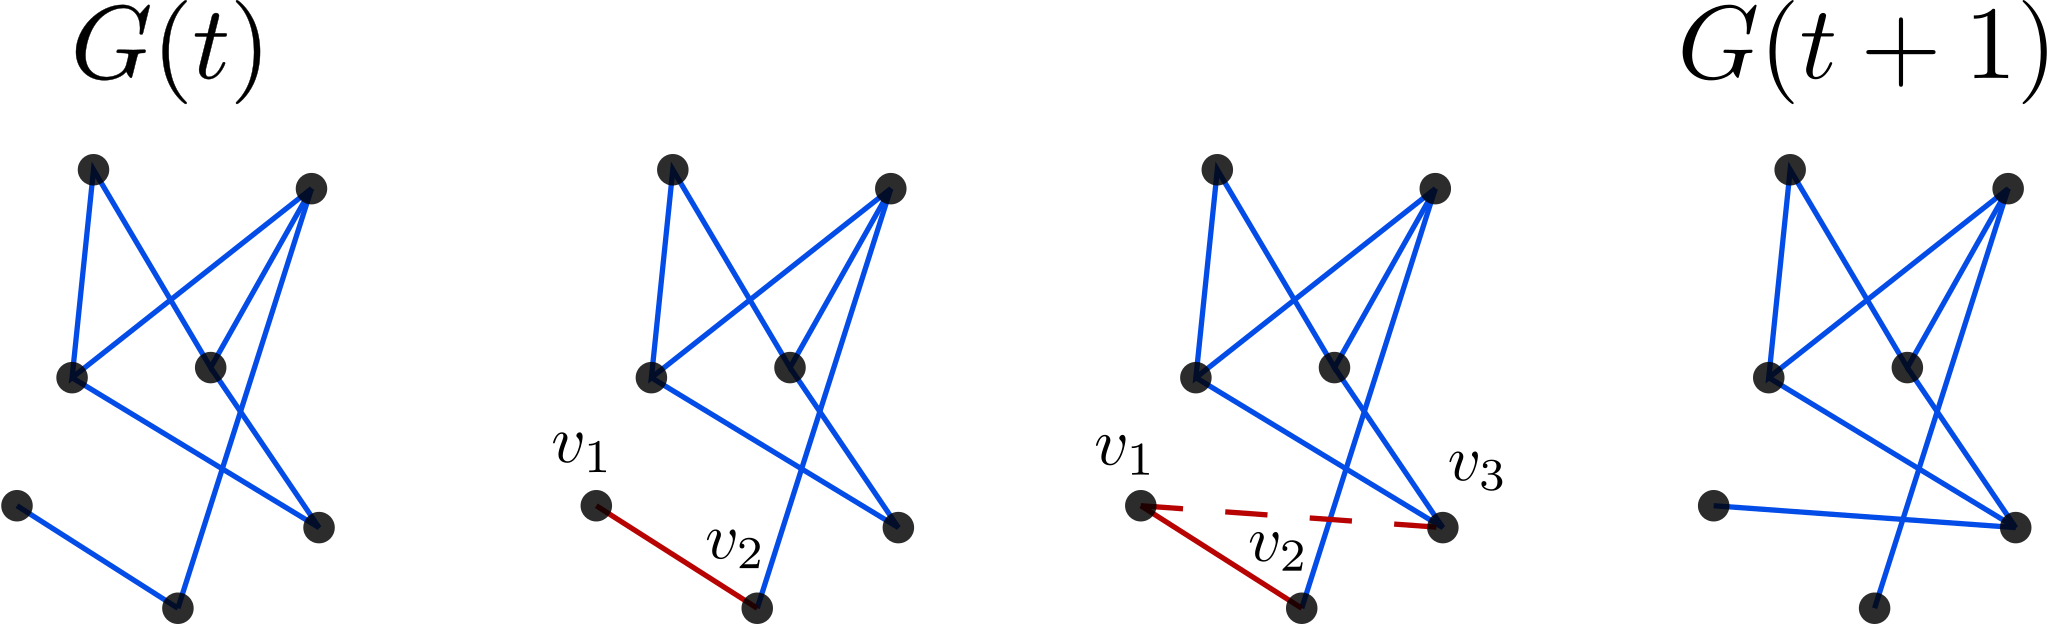
\includegraphics[width=0.9\textwidth]{graph-evo}
    \caption[Schematic of the substeps involved in the multigraph
    evolution dynamics]{Schematic of the substeps of the evolution
      dynamics of the multigraph
      $G(t)$. \label{fig:step-illustration}}
  \end{figure}

  \begin{figure}
    \vspace{-5mm} \centering
    \begin{subfigure}[t]{0.49\textwidth}
      \centering
      \includegraphics[width=\textwidth]{lopsided-degs-a}
      \subcaption{\label{fig:lopsided-init}}
    \end{subfigure} %
    \begin{subfigure}[t]{0.49\textwidth}
      \centering
      \includegraphics[width=\textwidth]{erdos-degs-a}
      \subcaption{\label{fig:erdos-init}}
    \end{subfigure}
    \caption[Evolution of the multigraph model's sorted degree
    sequence]{Evolution of the multigraph model's sorted degree
      sequence. Two distinct transients are shown, initialized with
      (a) an Erd\H{o}s-R\'{e}nyi random graph with $m = 5,050$ edges
      and (b) a graph in which half the vertices are isolated, and
      half uniformly share $m = 5,050$ edges. Both approach the same
      ultimate stationary sequence. To smoothen the evolution of this
      stochastic system, here we plot the instantaneous average of
      twenty simulations. \label{fig:dse}}
  \end{figure}

  \begin{figure}
    \centering
    \includegraphics[width=0.8\textwidth]{triangle-slaving-n2-n3}
    \caption[Evolution of triangle count]{Evolution of higher-order
      network statistics (here, the total triangle count) for three
      different network initializations. They are quickly ($O(n^2)$
      steps) drawn to a slow manifold on which they slowly evolve over
      ($O(n^3)$ steps) to a stationary state. \label{fig:sv}}
  \end{figure}

  \section{Equation-free modeling\label{sec:ef}}

  \subsection{Coarse-graining}

  A prerequisite to the implementation of equation-free algorithms is
  the determination of those few, select variables with which one can
  ``close'' a useful approximate description of the coarse-grained
  dynamics of the full, detailed network.
  % 
  This set of variables should clearly be (much) less than those of
  the full system state, and they should evolve smoothly (so, either
  our network would have a large number of nodes, or we would take
  expectations over several realizations of networks with the same
  collective features).
  % 
  Based on the profiles depicted in Fig. (\ref{fig:dse}), the graph's
  degree sequence, (equally informatively, its degree distribution) is
  a good candidate collective observable.
  % 
  It appears to evolve smoothly, while also providing significant
  savings in dimensionality, from an $O(n^2)$ adjacency matrix to a
  length-$n$ vector of degrees. \par

  It now becomes crucial to test whether the evolution of other
  properties of the graph can be correlated to the degree sequence.
  % 
  If not, our current description is incomplete (an equation cannot
  close with only the degree sequence) and there exist other important
  coarse variables that must be included in our macroscopic system
  description.
  % 
  To assess this, we constructed graphs with identical degree
  sequences but varying triangle counts and recorded the evolution of
  this observable under the dynamics prescribed in Section
  \ref{sec:m}. Fig. (\ref{fig:sv}) shows that, within a short time,
  the triangle counts are drawn to an apparent shared ``slow
  manifold'', despite the variation in initial conditions.
  % 
  This supports our selection of the degree sequence as an adequate
  coarse variable to model the system. \par

  Next we describe the other two key elements to equation-free
  modeling which map to and from our microscopic and macroscopic
  descriptions: restriction and lifting operators.

  \begin{figure}
    \centering
    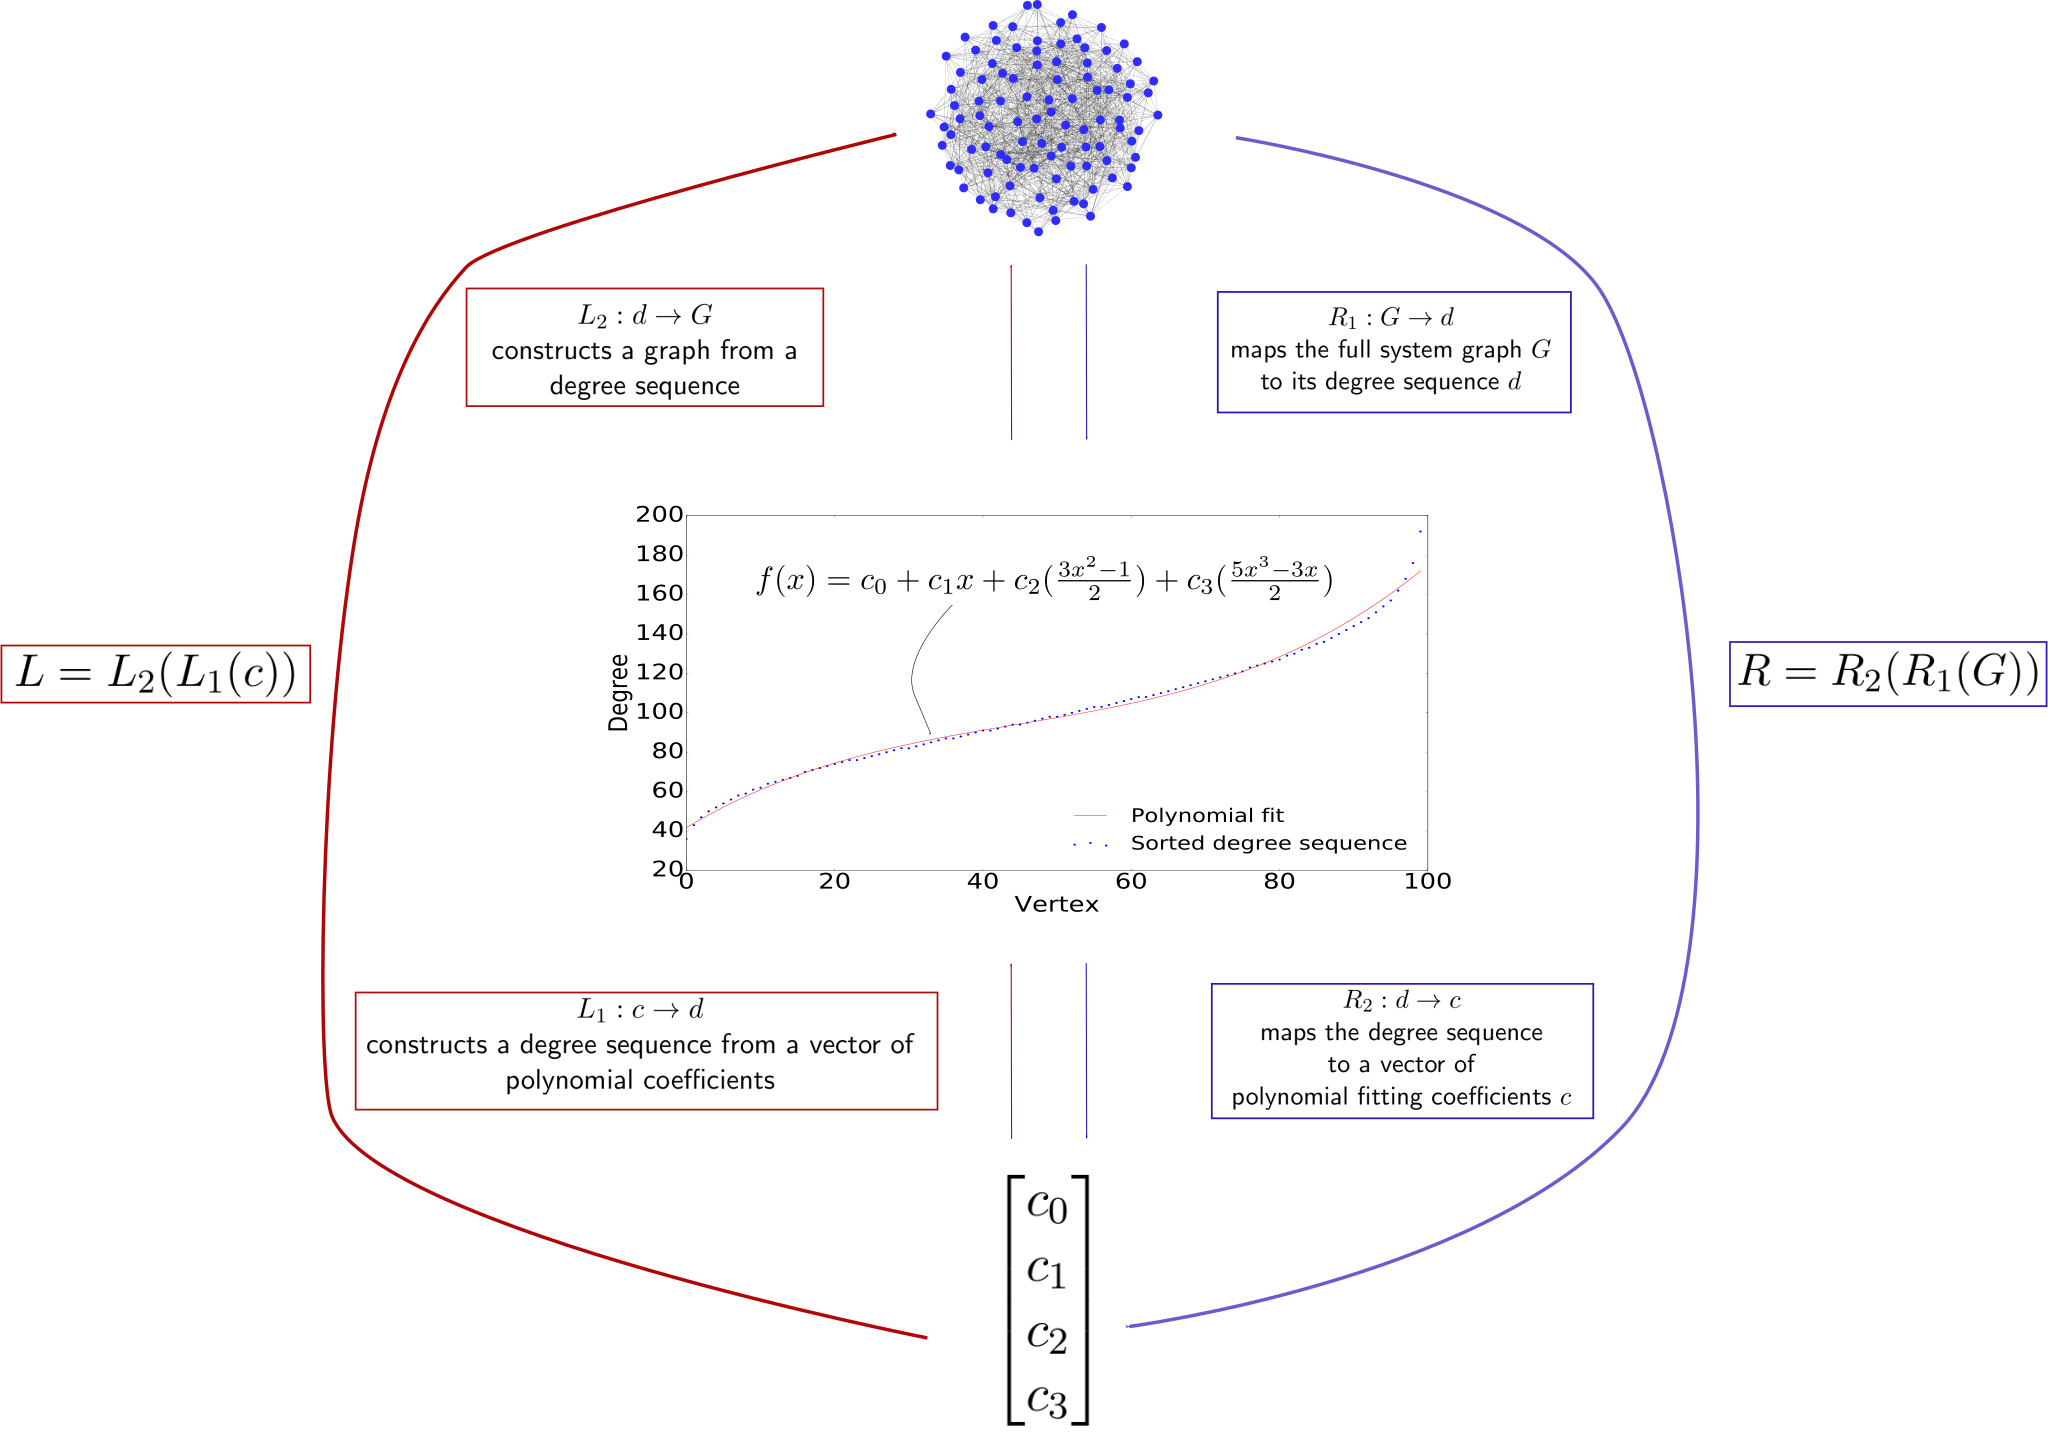
\includegraphics[width=\textwidth]{cpi-diagram}
    \caption[Schematic of multigraph's lifting and restricting
    procedures]{Schematic of our restriction ($\Res$) and
      lifting ($\Li$) procedures. The graph's sorted degree
      sequence is calculated ($R_1$) and then fit to a third-order
      polynomial ($R_2$). This maps graphs ($G$) to vectors of four
      coefficients ($\mathbf{c}$). To lift, the polynomial is used to
      generate a degree sequence ($L_1$), which is then used to
      construct a consistent graph ($L_2$). This process maps vectors
      of four coefficients ($\mathbf{c}$) to graphs ($G$).
      $\Res = R_2 \circ R_1 $ is our restriction and
      $\Li = L_2 \circ L_1$ is our
      lifting. \label{fig:cpi-diagram}}
  \end{figure}


  \subsection{Restriction}

  The restriction operator ``translates'' the full network description
  to its corresponding coarse variable values.
  % 
  Here, this involves mapping a multigraph to its sorted degree
  sequence, a simple calculation.
  % 
  However, we may be able to further reduce the dimensionality of our
  coarse system by keeping not the entire length-$n$ degree sequence,
  but rather a low-order polynomial fitting of it.
  % 
  To do so, we first sort the sequence to achieve a smooth,
  monotonically increasing dataset, then fit the result to a
  third-order polynomial, which had been observed to closely
  approximate the sequence evolution throughout time.
  % 
  Our coarse description thus consisted, at every moment in time, of
  the four polynomial coefficient values, specifying a particular
  sorted degree sequence, as shown in Fig. (\ref{fig:cpi-diagram}).
  % 
  The restriction operator therefore maps multigraphs to length-four
  coefficient vectors.
  % 
  This procedure is represented by the blue arrows of
  Fig. (\ref{fig:cpi-diagram}).

  \subsection{Lifting}

  The lifting operator performs the inverse role of restriction:
  translating coarse variables into full networks.
  % 
  This is clearly a one-to-many mapping.
  % 
  Specifically in the context of our model, we map vectors of
  polynomial coefficients to full networks in a two-stage process.
  % 
  First, the coefficient vector is used to recreate a sorted degree
  sequence by evaluating the full polynomial at integer values and
  rounding to the nearest degree, as depicted in
  Fig. (\ref{fig:cpi-diagram}).
  % 
  If the sum of the resulting degree sequence is odd, a single degree
  is added to the largest value to ensure the sequence is graphical.
  % 
  Second, this degree sequence is used as input to any algorithm that
  produces a network consistent with a graphical degree sequence (here
  we typically used a Havel-Hakimi algorithm, creating a graph whose
  degree sequence matches that of the input
  \cite{havel_remark_1955,hakimi_realizability_1962}).
  % 
  While the canonical Havel-Hakimi method produces simple graphs, it
  is not difficult to extend it to multigraphs by allowing the
  algorithm to wrap around the sequence, producing multiple edges and
  self-loops.  The lifting procedure is represented by the red arrows
  of Fig. (\ref{fig:cpi-diagram}).

  \subsection{Coarse projective integration (CPI)}
  \label{sec:cpi}

  The components described above are combined to accelerate
  simulations through Coarse Projective Integration.
  % 
  Denoting the lifting operator by
  $\Li \; : \; c \rightarrow G$ where $c \in \mathbb{R}^4$ is
  the vector of polynomial coefficients, and the restriction operator
  as $\Res \; : G \rightarrow c$, the algorithm progresses as
  follows:

  \begin{enumerate}
  \item Advance the full system for $t_h$ steps
    \label{cpi:heal}
  \item Continue for $t_c$ steps, restricting the network at intervals
    and recording the coarse variable values
  \item Using the coarse variables collected over the previous $t_c$
    steps, project each variable forward $t_p$ steps with, here, a
    forward-Euler method
    \label{cpi:proj}
  \item With the new, projected coarse variables, lift to one (or more
    copies of) full network
    \label{cpi:init}
  \item Repeat from Step (\ref{cpi:heal}) until the desired time has
    been reached.
  \end{enumerate}

  Note that Step (\ref{cpi:heal}) is intended to allow a singularly
  perturbed quantity to approach its slow manifold.
  % 
  Upon initializing a new full system (here, a new network) in Step
  (\ref{cpi:init}), higher order observables (for example, the
  triangle count) will be far from the values they would attain in a
  detailed simulation.
  % 
  If the coarse system model closes with our chosen variables, then
  either (a) these quantities do not affect the dynamics of the degree
  sequence; or (b) they do, but then by hypothesis these quantities
  quickly evolve to functions of the selected coarse variables (i.e.,
  they approach the slow manifold).
  % 
  In the second case, after a short interval of ``healing'' they will
  be drawn to the expected trajectory, after which we begin sampling.
  % 
  This is analogous to Fig. (\ref{fig:sv}).
  % 
  The computational gains arise from the projective step,
  (\ref{cpi:proj}).
  % 
  Here, we advance the system $t_p$ steps at the cost of one
  evaluation of forward Euler, instead of $t_p$ direct detailed steps.

  Results of the application of this general framework with the
  specific lifting and restriction operators previously outlined are
  shown in Fig. (\ref{fig:cpi-results}). We used an $n=100$-vertex
  graph with $m=50000$ edges and parameter value $\kappa=1$. We ran
  the model for a total of $10 \cdot n^3$ steps, with
  $t_h = 10 \cdot n^2$, $t_c = n^3$ and $t_p = 50 \cdot n^2$.
  % 
  We see good agreement between the CPI-accelerated and normal
  systems, while reducing the number of detailed steps by one third.
  % 
  It is important to mention that this method was applied not to a
  single system instantiation, but to an ensemble of fifty such
  realizations.  This ensured that when properties such as the fitted
  polynomial coefficients were averaged over the ensemble they evolved
  smoothly despite the stochastic nature of the system; in effect, we
  are computing the ``expected network evolution'' averaged over
  consistent realizations.

  \begin{figure}
    \vspace{-5mm} \centering
    \begin{subfigure}{0.59\textwidth}
      \centering
      \includegraphics[width=\textwidth]{cpi-3d-comp-stretch}
      \subcaption{\label{fig:cpi-error}}
    \end{subfigure} %
    \begin{subfigure}{0.39\textwidth}
      \centering
      \includegraphics[width=\textwidth]{cpi-relative-error-n3}
      \subcaption{\label{fig:self-error}}
    \end{subfigure}%
    \caption[Coarse-projective integration results]{CPI results: (a)
      the evolution of the CPI-accelerated degree sequence (red)
      compared to direct simulation (blue) and (b) error in
      CPI-accelerated runs calculated by comparing CPI-accelerated
      degree sequences to those arising from an ensemble of direct
      simulations. \label{fig:cpi-results}}
  \end{figure}


  \section{Coarse Newton-GMRES}
  \label{sec:ng}
  Aside from the computational savings of model simulations offered by
  CPI, the equation free framework also permits the calculation of
  system steady states through fixed point (here, matrix-free
  Newton-GMRES) algorithms.
  % 
  Referring back to the CPI procedure outlined in
  Sec. (\ref{sec:cpi}), we can define an operator
  $\Theta: \mathbf{d} \rightarrow \mathbf{d}$ projecting coarse
  variables at $t$ to their values at $t + \delta t$:
  $\mathbf{d}(t+\delta t) =\Theta(\mathbf{d}(t))$.
  % 
  Note that in this section, we take the sorted degree sequence as our
  coarse variable.
  % 
  A system fixed point could then be located by employing Newton's
  method to solve the equation

  \begin{align}
    \label{eq:f}
    \mathbf{F}(\mathbf{d}) \equiv \Theta(\mathbf{d}) - \mathbf{d} = 0
  \end{align}

  However, this requires the repeated solution of the system of linear
  equations
  $DF(\mathbf{d}^{(k)}) \cdot \delta \mathbf{d}^{(k+1)} =
  -\mathbf{F}(\mathbf{d}^{(j)})$, in which the system Jacobian, $DF$
  is unavailable.
  % 
  Thankfully, we may circumvent this obstacle by estimating the
  directional derivatives $DF(\mathbf{d}) \cdot \delta \mathbf{d}$ via
  a difference approximation of the form

  \begin{align}
    DF(d) \cdot \delta \mathbf{d} \approx \frac{\| \delta \mathbf{d} \| \mathbf{F}(\mathbf{d} + h \| \mathbf{d} \| \frac{\delta \mathbf{d}}{\| \delta \mathbf{d} \|}) - \mathbf{F}(\mathbf{d})}{h \| \mathbf{d} \|}
  \end{align}

  \noindent for nonzero $\mathbf{d}$, which in turn is evaluated
  through calls to $\mathbf{F}$ as defined in Eq. (\ref{eq:f})

  This is precisely the approach of the Newton-GMRES method, in which
  the solution to a linear system is sought for in expanding Krylov
  subspaces \cite{kelley_solving_2003}.
  % 
  Applying this algorithm in conjunction with the $\Theta$ operator
  defined in Sec. (\ref{sec:cpi}) allowed us to locate the stationary
  distribution without simply running and observing the full system
  for long times, as would otherwise be required.
  % 
  Results are shown in Fig. (\ref{fig:newton-results}).
  % 
  We note that coarse stability results can also be obtained via an
  iterative Arnoldi eigensolver, again estimating matrix-vector
  products as above.

  \begin{figure}
    \vspace{-5mm} \centering
    \begin{subfigure}{0.49\textwidth}
      \centering
      \includegraphics[width=\textwidth]{newton-error}
      \subcaption{\label{fig:newton-error}}
    \end{subfigure} %
    \begin{subfigure}{0.49\textwidth}
      \centering
      \includegraphics[width=\textwidth]{newton-comp}
      \subcaption{\label{fig:newton-comp}}
    \end{subfigure}%
    \caption[Coarse Newton-GMRES results]{Coarse Newton-GMRES results:
      (a) evolution of the error in the coarse Newton-GMRES iteration
      scheme; and (b) visual comparison of the algorithm's solution to
      the stationary state obtained from direct
      simulation. \label{fig:newton-results}}
  \end{figure}


  \section{Algorithmic coarse-graining}
  \label{sec:dr}
  Crucial to the above analysis was the determination of suitable
  coarse, system variables: it is the starting point of any equation
  free method.
  % 
  However, the discovery of such a low-dimensional description is
  highly non-trivial.
  % 
  Currently, as in this paper, they are ``discovered through informed
  experience'': through careful investigation of direct simulations,
  and knowledge of previous analytical results.
  % 
  Clearly, any process which could algorithmically guide this search
  based on only simulation data would be of great benefit to the
  modeling practitioner.
  % 
  We now illustrate two such algorithms: principal component analysis
  (PCA) and diffusion maps (DMAPS).
  % 
  First, we briefly discuss some aspects of the important issue of
  defining distances between networks, a prerequisite for any
  dimensionality-reduction technique.

  \subsection{On network distances}

  When applying dimensionality reduction techniques to a dataset, it
  is necessary to define a distance (or similarity) between each pair
  of data points.
  % 
  If these points are a set of vectors in $\mathbb{R}^n$ one has a
  number of metrics to choose from, the Euclidean distance being a
  common first option.
  % 
  Unfortunately, when individual points are not vectors but networks,
  the definition of a useful and computationally easily quantified
  metric becomes far more challenging.
  % 
  Examples such as the maximal common subgraph and edit distances,
  defined in \cite{bunke_graph_1998} and \cite{gao_survey_2010} define
  metrics on the space of graphs, but their computation is
  $NP\textnormal{-}hard$.
  % 
  Other computationally feasible approaches include comparing
  distributions of random walks on each graph
  \cite{vishwanathan_graph_2010}, calculating the so-called $n$-tangle
  density \cite{gallos_revealing_2014}, or calculating the edit
  distance
  with an approximation algorithm \cite{riesen_approximate_2009,zeng_comparing_2009}.

  The strategy used in the following computations, detailed in
  \cite{rajendran_analysis_2013} and \cite{xiao_structure-based_2008},
  enumerates the number of times a certain set of motifs (or
  subgraphs) appears in each network in the dataset.
  % 
  This maps each network to a vector in $\mathbb{R}^n$, and the
  Euclidean distance is subsequently used to quantify the similarity
  of two graphs.
  % 
  Due to computational restrictions, we chose here to only count the
  number of three- and four-vertex single-edge subgraphs contained in
  each network.
  % 
  As there are eight such motifs, shown in Fig. (\ref{fig:motifs}),
  this process $\gamma$ maps each graph to an eight-dimensional
  vector: $\gamma : G \rightarrow \mathbb{R}^8$.
  % 
  We applied this operation to a simplified version of each graph,
  wherein any multiple edges were reduced to a single edge.

  \begin{figure}
    \vspace{-5mm} \centering
    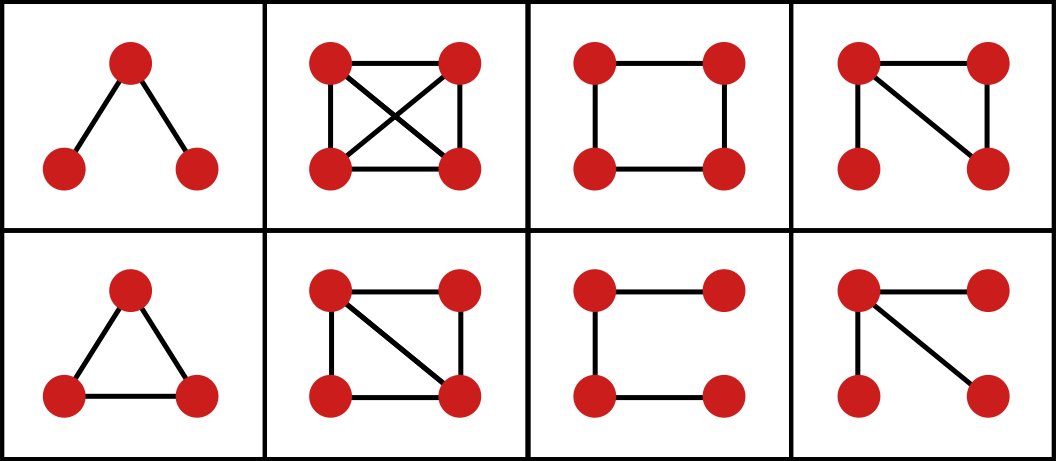
\includegraphics[width=\textwidth]{motifs}
    \caption[List of subgraphs used to embed multigraphs]{List of the
      single-edge subgraphs used to embed each network.  The number of
      times each appeared in the simplified input graph was
      calculated, mapping input graphs to
      $\mathbb{R}^8$. \label{fig:motifs}}
  \end{figure}

  \subsection{PCA\label{sec:pca}}
  

  PCA is used to embed data into linear subspaces that capture the
  directions along which the data varies most
  \cite{jolliffe_principal_2014}.
  % 
  Given some matrix $X \in \mathbb{R}^{n \times m}$ in which each of
  the $m$ column vectors $x_i$ represents a different collection of
  the $n$ system variables (i.e. a different data point), PCA computes
  a reduced set of $k<n$, orthogonal ``principal components''
  $z_i \in \mathbb{R}^n$ that constitute an optimal basis for the data
  in the sense that, among linear, $k$-dimensional embeddings,
  $w_i = Z^Tx_i$ captures the maximum possible variance in the
  dataset, where
  $Z = \begin{bmatrix} | & | & & | \\ z_1 & z_2 & \hdots & z_k \\ | &
    | & & | \end{bmatrix}$.
  % 
  This approach has found wide application, but can suffer from its
  inability to uncover simple \textit{nonlinear} relationships among
  the input variables.
  % 
  Indeed, many datasets will not ``just lie along some hyperplane''
  embedded in $\mathbb{R}^n$, but will rather lie on a low-dimensional
  nonlinear manifold throughout the space.

  Theoretical results in \cite{rath_time_2012} state that, for a given
  network size $n$, the final stationary state depends only on the
  number of edges present $m$ and the model parameter $\kappa$.
  % 
  To assess both the validity of our graph embedding technique and the
  usefulness of PCA in the context of complex networks, we generated a
  dataset of stationary states over a range of $m \in [50, 5000]$ and
  $\log(\kappa) \in [0, 2]$ values by directly running the model over
  $2n^3$ steps ($N=30$ values of each parameter were taken, for a
  total of $900$ networks).
  % 
  We fixed the network size to $n=50$ vertices.
  % 
  Each resulting graph $G(m_i, \kappa_j) = G_{ij}$ was then embedded
  into $\mathbb{R}^8$ by counting the number of times each of the
  subgraphs shown in Fig. (\ref{fig:motifs}) appeared in the network.
  % 
  Thus $\gamma(G_{ij}) = v_{ij} \in \mathbb{R}^8$.
  % 
  We then proceeded to perform a principal component analysis on this
  collection of vectors $\{v_{ij}\}_{i,j=1}^N$.
  % 
  Interestingly, the first two principal components $z_1$ and $z_2$
  succeeded in uncovering a two-dimensional embedding of the dataset
  corresponding to the two underlying parameters $m$ and $\kappa$, as
  shown in Fig. (\ref{fig:pca}) in which the data is projected on the
  plane spanned by these two vectors.
  % 
  This suggests that, given some final network state $G(m, \kappa)$,
  by projecting its embedding onto these first two principal
  components one could obtain a reasonable approximation of the hidden
  parameter $\kappa$.

  \begin{figure}
    \vspace{-5mm} \centering
    \begin{subfigure}{0.49\textwidth}
      \centering
      \includegraphics[width=\textwidth]{pca-2d-rho-a}
      \subcaption{\label{fig:pca-rho}}
    \end{subfigure} %
    \begin{subfigure}{0.49\textwidth}
      \centering
      \includegraphics[width=\textwidth]{pca-2d-kappa-a}
      \subcaption{\label{fig:pca-kappa}}
    \end{subfigure}%
    \caption[Principal component analysis of motif-based
    embeddings]{PCA of motif-based embeddings: (a) coloring the
      two-dimensional PCA embedding with $\rho$ and (b) coloring the
      two-dimensional PCA embedding with $\kappa$. \label{fig:pca}}
  \end{figure}

  \subsection{Diffusion Maps}

  Unlike PCA, DMAPS uncovers parameterizations of nonlinear manifolds
  hidden in the data.
  % 
  This is achieved by solving for the discrete equivalent of the
  eigenfunctions and eigenvalues of the Laplace-Beltrami operator over
  the manifold, which amounts to calculating leading
  eigenvector/eigenvalue pairs of a Markov matrix $A$ describing a
  diffusion process on the dataset.
  % 
  As the eigenfunctions of the Laplace-Beltrami operator provide
  parameterizations of the underlying domain, the output eigenvectors
  $\Phi_i$ from DMAPS similarly reveal and parameterize any hidden
  nonlinear structure in the input dataset. The $k$-dimensional DMAP
  of point $x_i$ is given by

  \begin{align*}
    \Psi(x_i; t) = \begin{bmatrix} \lambda_1^t \Phi_1(i) \\ \lambda_2^t
      \Phi_2(i) \\ \vdots \\
      \lambda_k^t \Phi_k(i) \end{bmatrix}
  \end{align*}

  \noindent where $\lambda_i$ is the $i^{th}$ eigenvalue of the Markov
  matrix $A$, $\Phi_i(j)$ the $j^{th}$ entry of eigenvector $i$, and
  the parameter $t$ allows one to probe multiscale features in the
  dataset. See \cite{coifman_diffusion_2006,nadler_diffusion_2006} for
  further details.

  First we applied DMAPS to the dataset described in
  Sec. (\ref{sec:pca}).
  % 
  Given the apparent success of PCA in this setting, one would expect
  DMAPS to also uncover the two-dimensional embedding corresponding to
  different values of $m$ and $\kappa$.
  % 
  Fig. (\ref{fig:dmaps-rk}) shows that this is indeed the case: using
  $\Phi_1$ and $\Phi_4$ to embed the graphs produces a two-dimensional
  surface along which both $\rho$ and $\kappa$ vary independently.

  Additionally, we were interested in embeddings of different model
  trajectories.
  % 
  This dataset was generated by sampling two different model
  simulations as they evolved ($N=2000$ points were sampled from each
  trajectory).
  % 
  The parameters $n$, $m$ and $\kappa$ were held constant at $200$,
  $20100$ and $1.0$ respectively, but one graph was initialized as an
  Erd\H{o}s-R\'{e}nyi random graph (Fig. (\ref{fig:erdos-init})),
  while the other was initialized as a ``lopsided'' graph
  (Fig. (\ref{fig:lopsided-init})).
  % 
  Every $500$ steps the graph would be recorded till $N$ snapshots
  were taken of each trajectory, for a total of $1000000$ steps.
  % 
  Letting $G_e(t)$ refer to the Erd\H{o}s-R\'{e}nyi-initialized system
  at step $t$, and $G_l(t)$ the lopsided-initialized system, the
  embedding $\gamma$ was used to create points
  $\gamma(G_e(t)) = v_e(t) \in \mathbb{R}^8$ and
  similarly $\gamma(G_l(t)) = v_l(t) \in \mathbb{R}^8$.

  DMAPS was then applied to this set of $2N$ points, and the
  three-dimensional embedding using $\Phi_1$, $\Phi_2$ and $\Phi_3$ is
  shown in Fig. (\ref{fig:dmaps-results}).
  % 
  At first, the two trajectories are mapped to distant regions in
  $\mathbb{R}^3$ due to their different initial conditions.
  % 
  They evolve along different ``regions'' of the embedding, taking two
  distinct trajectories on their approach to the stationary state.
  % 
  Eventually, their embeddings meet as they arrive at this final,
  shared state, each asymptotically along opposite sides of the
  slowest eigenvector of the linearization of the steady state.
  % 
  DMAPS thus proves useful in elucidating both geometric and dynamic
  features of the system as shown in Figs. (\ref{fig:dmaps-rk}) and (\ref{fig:dmaps-results}).

  We see that both PCA and DMAPS, when combined with a suitable
  embedding of each graph, can help uncover useful information
  pertaining to the underlying dimensionality of the problem dynamics.


  \begin{figure}
    \vspace{-5mm} \centering
    \begin{subfigure}{0.49\textwidth}
      \centering
      \includegraphics[width=\textwidth]{dmaps-2d-rho-a}
      \subcaption{\label{fig:dmaps-rho}}
    \end{subfigure} %
    \begin{subfigure}{0.49\textwidth}
      \centering
      \includegraphics[width=\textwidth]{dmaps-2d-kappa-a}
      \subcaption{\label{fig:dmaps-kappa}}
    \end{subfigure}%
    \caption[DMAP of motif-based embeddings when system parameters are
    varied]{DMAP of motif-based embeddings from a collection of
      simulations run at different parameter values: (a) coloring the
      two-dimensional DMAPS embedding with $\rho$ and (b) coloring the
      two-dimensional DMAPS embedding with $\kappa$. As with PCA,
      DMAPS uncovered the parameters governing the stationary state,
      known from \cite{rath_time_2012} \label{fig:dmaps-rk}}
  \end{figure}

  \begin{figure}
    \vspace{-5mm} \centering
    \begin{subfigure}{0.49\textwidth}
      \centering
      \includegraphics[width=\textwidth]{dmaps-3d-convergence-a}
      \subcaption{\label{fig:dmaps-results-regular}}
    \end{subfigure} %
    \begin{subfigure}{0.49\textwidth}
      \centering
      \includegraphics[width=\textwidth]{dmaps-3d-convergence-zoom-a}
      \subcaption{\label{fig:dmaps-results-zoom}}
    \end{subfigure}%
    \caption[DMAP of motif-based embeddings when two trajectories are
    sampled]{DMAP of motif-based embeddings from two separate
      simulation trajectories: (a) embedding of two trajectories
      starting from different initial conditions. While the
      trajectories are initially mapped to separate regions of
      ``embedding space'', they eventually evolve to the same coarse
      stationary state.  Final states are circled, and point size
      grows as more steps are taken in each trajectory.  (b) Enlarged
      view of the final points in the previous plot, revealing the
      approach to a similar final state along opposite sides of the
      slowest eigenvector of its linearization.  Here, the average of
      the final fifty points is circled. Due to the stochastic nature
      of the system, the final embeddings mildly fluctuate randomly
      about the shared stationary state. \label{fig:dmaps-results}}
  \end{figure}

  \section{Conclusion}

  The equation free framework was successfully applied to the
  edge-conservative preferential attachment model, accelerating
  simulations through CPI and locating stationary states through
  coarse Newton-GMRES. This indicates potential avenues for improving
  simulation times of other complex network models, such as those
  found in epidemiology.
  % 
  Additionally, an underlying two-dimensional description was
  uncovered via PCA and DMAPS. These automated methods of
  dimensionality-reduction are quite general, and can in principle be
  applied in a wide range of network settings to probe hidden
  low-dimensional structure. For an application in the setting of
  labeled nodes, see ({\cite{kattis_modeling_2016}}).

  However, an open area of investigation is the interpretation of the
  output from the PCA and DMAPS techniques.
  % 
  As a linear map, PCA retains a clear relationship between its input
  and output, but is less effective when data lie on highly nonlinear
  manifolds.
  % 
  DMAPS may perform better the task of dimensionality reduction, but
  it is unclear how the embedding coordinates relate to physical
  features of the sampled networks.
  % 
  While this approach opens several promising avenues in
  coarse-graining complex network dynamics, it also reveals two
  ``bottlenecks'' for the process: (a) the selection of informative
  and practically computable graph distance metrics, necessary in the
  discovery of good coarse variables; and (b) the construction of
  network realizations consistent with (conditioned on) specific
  values of collective observables.
  % 
  Both items are, and we expect will continue being, the subject of
  intense investigation by many research groups, including ours.


%%% Local Variables: ***
%%% mode:latex ***
%%% TeX-master: "../../thesis.tex"  ***
%%% End: ***